
%%%%%%%%%%%%%%%%%%%%%%%%%%%%%%%%%%%%%%%%%%%%%%%%%%%%%%%%%%%%%%%%%%%%%%%%%%%%%%%
\section[Probability theory]{Probability Theory Overview}
\miniframesoff
\begin{frame}
    \tableofcontents[currentsection]
\end{frame}
\miniframeson
%%%%%%%%%%%%%%%%%%%%%%%%%%%%%%%%%%%%%%%%%%%%%%%%%%%%%%%%%%%%%%%%%%%%%%%%%%%%%%%

%%%%%%%%%%%%%%%%%%%%%%%%%%%%%%%%%%%%%%%%%%%%%%%%%%%%%%%%%%%%%%%%%%%%%%%%%%%%%%%%
\begin{frame}{Probabilistic event}

Consider flipping a fair coin. There are two possible outcomes: 

\begin{itemize}
    \item $H$: Flip heads
    \item $T$: Flip tails
\end{itemize}

\onslide<2->
\vspace{2ex}
This is a \alert<2>{probabilistic event}; there's some uncertainty in what the outcome is. 


\vspace{2ex}
\onslide<3->
Suppose we have a fair coin. I flip it. What is the probability $\PP (\cdot)$ of the following events?:
\begin{itemize}
    \item $\PP (H)$? (i.e. probability of flipping heads)
    \onslide<4->
    \item $\PP (T)$? (i.e. probability of flipping tails?)
    \onslide<5->
    \item $\PP (H \text{ OR } T)$? Also referred to as $\PP (H \cup T)$
    \onslide<6->
    \item Of flipping neither heads nor tails?
    \onslide<7-> 
    \item $\PP (H \text { AND } T)$? Also referred to as $\PP (H \cap T)$ or $\PP (H, T)$ (remember, there's only one coin flip)
\end{itemize}

\vspace{2ex}
\onslide<8->
Another example: suppose we roll a fair die. The possible outcomes are rolling $\{1, 2, 3, 4, 5, 6\}$.
\begin{itemize}
    \onslide<9->
    \item What is the probability of rolling a 2?
    \onslide<10->
    \item What is the probability of rolling a 2 or a 3?
\end{itemize}

\end{frame}

%%%%%%%%%%%%%%%%%%%%%%%%%%%%%%%%%%%%%%%%%%%%%%%%%%%%%%%%%%%%%%%%%%%%%%%%%%%%%%%%
\begin{frame}{Axioms of probability}

Probability measures are represented as a function $\PP(\cdot)$, and follow a few rules:
\begin{enumerate}
    \item Let the universe of possible outcomes be represented by $\Omega$. Then:
    \begin{equation*}
        \PP (\Omega) = 1
    \end{equation*}
    \pause
    \begin{itemize}
        \item[$\implies$] In our coin example, I'll either flip a heads or a tails, meaning $\Omega = \{H, T\}$. This law means that if I flip a coin, the probability that it comes up heads, or comes up tails, equals 1
    \end{itemize}
    \pause
    \item Probabilities are less than zero and greater than one. So for some possible outcome A:
    \begin{equation*}
        0 \leq \PP (A) \leq 1
    \end{equation*}
    \pause
    \begin{itemize}
        \item[$\implies$] The probability of flipping a heads is $\PP (\text{Heads}) = \frac{1}{2}$
    \end{itemize}

    \pause
    \item When two events are \textbf{mutually exclusive} (they can't occur at the same time), you can add their probabilities:
    \pause
    \begin{itemize}
        \item Coin flip: $\PP (\text{Heads OR Tails}) = \PP (\text{Heads}) + \PP (\text{Tails}) $
        \item Die roll: $\PP (\text{Roll a 2 OR Roll a 3}) = \PP (\text{Roll a 2}) + \PP(\text{Roll a 3})$
    \end{itemize}

    For two mutually exclusive events $A_1$ and $A_2$:
    \begin{equation*}
        \PP (A_1 \cup A_2) = \PP (A_1) + \PP (A_2)
    \end{equation*}
    For $n$ mutually exclusive events $(A_1, A_2, \dots A_n)$:
    \begin{equation*}
        \PP \left( \cup_{i=1}^n A_i \right) \sum_{i=1}^n \PP (A_i)
    \end{equation*}
    
\end{enumerate}

\end{frame}

%%%%%%%%%%%%%%%%%%%%%%%%%%%%%%%%%%%%%%%%%%%%%%%%%%%%%%%%%%%%%%%%%%%%%%%%%%%%%%%%
\begin{frame}{Set terminology}

We often use set theory to describe probabilistic events. Consider the following outcomes of rolling a fair die:
\begin{equation*}
    A = \{\text{Roll an even number}\} = \{2, 4, 6\} \quad
    B = \{\text{Roll } \geq 4\} = \{4, 5, 6\} \quad
    C = \{\text{Roll } 1 \} = \{1\}
\end{equation*}
\begin{figure}
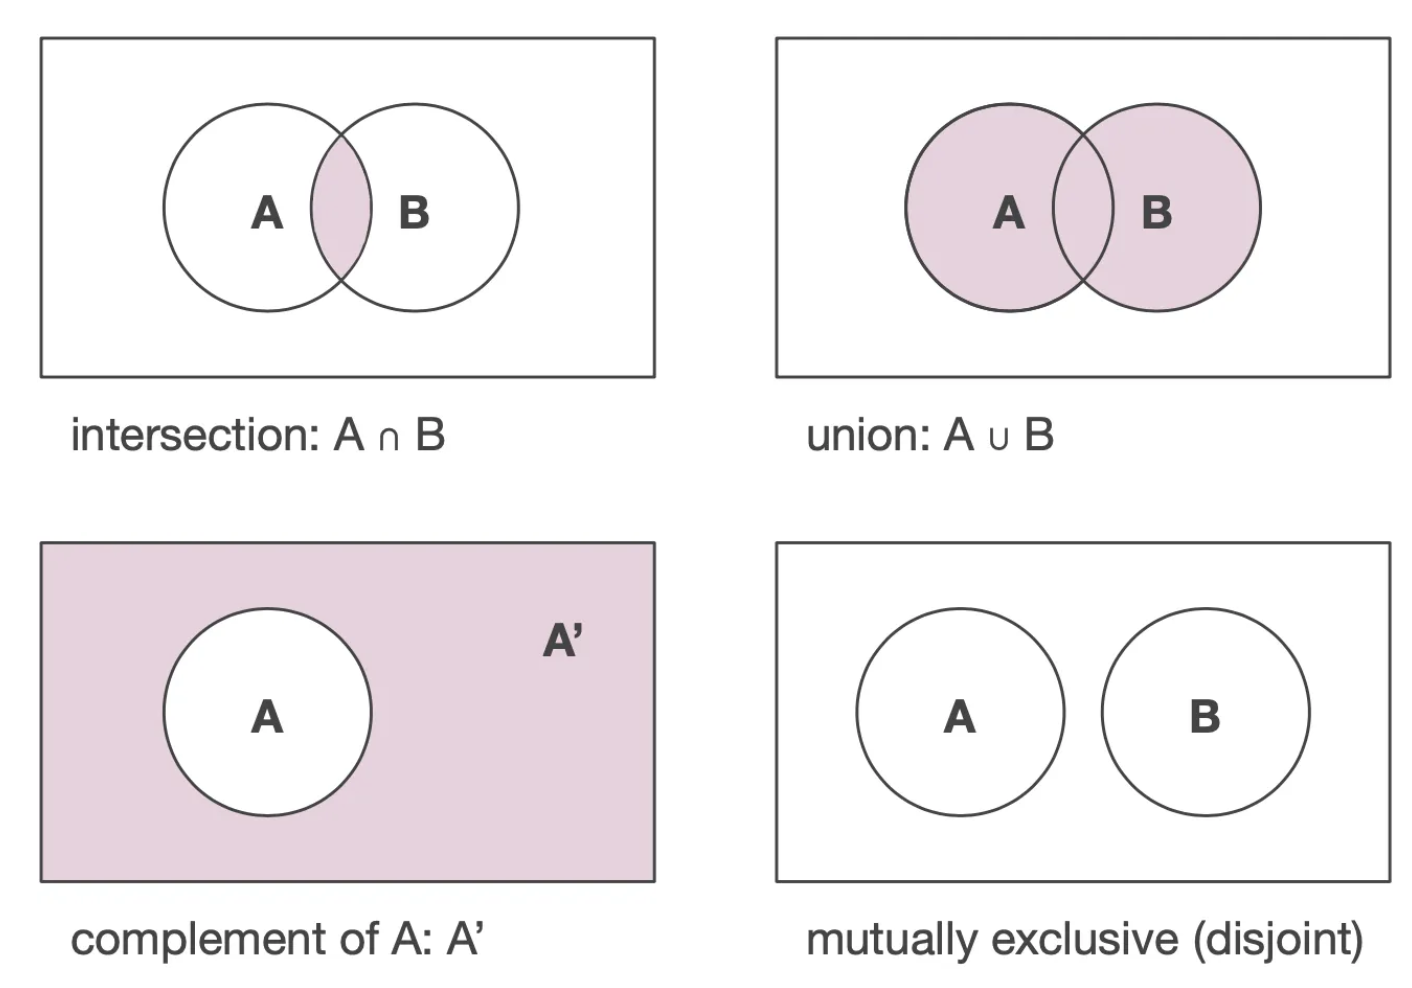
\includegraphics[scale=0.2]{img/sets.png}
\end{figure}

% \begin{itemize}
%     \item Intersection (AND): $A \cap B = \{2, 4, 6\} \cap \{4, 5, 6\} = \{4, 6\}$
%     \item Union (OR): $A \cup B = \{2, 4, 6\} \cup \{4, 5, 6\} = \{2, 4, 5, 6\}$
%     \item Complement (opposite): $A^C = \{2, 4, 6\}^C = \{1, 3, 5\}$
%     \item Mutually exclusive: $A$ and $A^C$ are mutually exclusive
% \end{itemize}

\begin{table}
\begin{tabular}{lrll}
Intersection &$A \cap B$&=$\{2, 4, 6\} \cap \{4, 5, 6\}$ &$=\{4, 6\}$ \\
Union &$A \cup B$&=$\{2, 4, 6\} \cup \{4, 5, 6\}$ &$=\{2, 4, 5, 6\}$ \\
Complement &$A^C$&=$\{2, 4, 6\}^C$ &$=\{1, 3, 5\}$ 
\end{tabular}
\end{table}
Question: are $A$ and $C$ mutually exclusive?

\end{frame}


%%%%%%%%%%%%%%%%%%%%%%%%%%%%%%%%%%%%%%%%%%%%%%%%%%%%%%%%%%%%%%%%%%%%%%%%%%%%%%%%
\begin{frame}{Probability Rules}

Several helpful rules follow from the aforementioned axioms.

\vspace{2ex}
\textbf{1. Complement Rule}: For any event A in the possible outcomes, the probabililty of A not happening (sometimes called the complement of $A$, or $A^C$) is:
\begin{equation*}
    \PP (\text{NOT } A) = \PP (A^C) = 1 - \PP(A)
\end{equation*}

\pause
\vspace{1ex}
\emph{Example: } You roll a die. The probability you roll a 2 is $\frac{1}{6}$:
\begin{equation*}
    \PP (\text{Roll a } 2) = \frac{1}{6}
\end{equation*}
What is the probability you roll either a 2, 3, 4, 5, or 6?

\pause
\emph{Answer: } Rolling a 2 is an event. The complement of this event is rolling a 2, 3, 4, 5, or 6:
\begin{align*}
    \PP (\{2, 3, 4, 5, 6\}) =& 1 - \PP (\{2\}) \\
    =& 1 - \frac{1}{6} \\
    =&\frac{5}{6}
\end{align*}

\vspace{1ex}
Practice: HW Question 1



\end{frame}


%%%%%%%%%%%%%%%%%%%%%%%%%%%%%%%%%%%%%%%%%%%%%%%%%%%%%%%%%%%%%%%%%%%%%%%%%%%%%%%%
\begin{frame}{Probability Rules (cont.)}


\textbf{2. Union of events}: For any events $A$ and $B$ (note: I'm not saying anything about these events being mutually exclusive): 
\begin{align*}
    \PP (A \text{ OR } B) = \PP (A \cup B) =& \PP (A) + \PP (B) - \PP (A \text{ AND } B) \\
    =& \PP (A) + \PP (B) - \PP (A \cap B)
\end{align*}

\pause
% \vspace{2ex}
\emph{Example}: When rolling a fair die, what is the probability of rolling an even number, or a number greater than or equal to 4?

% \vspace{2ex}
\emph{Answer}:
Define events $A$ and $B$ as:
\begin{equation*}
    A = \{\text{Roll an even number}\} = \{2, 4, 6\} \quad\quad
    B = \{\text{Roll } \geq 4\} = \{4, 5, 6\}
\end{equation*}
% Using the formula above:
% % \begin{align*}
% %     \PP (A) &= \PP (\{2, 4, 6\}) = \frac{1}{2} \\
% %     \PP (B) &= \PP (\{4, 5, 6\}) = \frac{1}{2} \\
% %     \PP (A \cap B) &= \PP (\{2, 4, 6\} \cap \{4, 5, 6\}) = \PP (\{4, 6\}) = \frac{1}{3} \\
% % \end{align*}
\vspace{2ex}
Finish on board. Practice: HW Question 2

\end{frame}

%%%%%%%%%%%%%%%%%%%%%%%%%%%%%%%%%%%%%%%%%%%%%%%%%%%%%%%%%%%%%%%%%%%%%%%%%%%%%%%%
\begin{frame}{Probability Rules (cont.)}

\textbf{3. Marginalization}

You can write the probability of any event $A$ in terms of $A \cap B$ and $A \cap B^C$. This is because $B$ and $B^C$ \textbf{partition} the universe of possible outcomes. Example:
\begin{align*}
    A &=\text{Rolling an even number} &&= \{2, 4, 6\} \\
    B &=\text{Rolling a number} \geq 4 &&= \{4, 5, 6\} \\
    B^C \onslide<2->{&&&= \{1, 2, 3\}}
\end{align*}
\onslide<3->
\begin{align*}
    \PP (A) &= \PP (A \cap B) + \PP (A \cap B^C) \\
    &= \PP (\{4, 6\}) + \PP (\{2\}) \\
    \onslide<4->{&= \frac{1}{3} + \frac{1}{6}}\onslide<5->{ = \frac{1}{2}}
\end{align*}
\onslide<6->
More generally, you can write $\PP (A)$ in terms of any sets $B_1, B_2, \dots, B_n$ that partition the universe of possible outcomes:
\begin{equation*}
    \PP (A) = \sum_{i=1}^n \PP (A \cap B_i) = \PP (A \cap B_1) + \PP (A \cap B_2) + \dots + \PP (A \cap B_n) 
\end{equation*}

\end{frame}

%%%%%%%%%%%%%%%%%%%%%%%%%%%%%%%%%%%%%%%%%%%%%%%%%%%%%%%%%%%%%%%%%%%%%%%%%%%%%%%%
\begin{frame}{Summary of probability rules (so far)}

\textbf{1. Complement Rule}: For any event A in the possible outcomes, the probability of A not happening (sometimes called the complement of $A$, or $A^C$) is:
\begin{equation*}
    \PP (\text{NOT } A) = \PP (A^C) = 1 - \PP(A)
\end{equation*}

\textbf{2. Union of events}: For any events $A$ and $B$ (note: I'm not saying anything about these events being mutually exclusive): 
\begin{align*}
    \PP (A \text{ OR } B) = \PP (A \cup B) =& \PP (A) + \PP (B) - \PP (A \text{ AND } B) \\
    =& \PP (A) + \PP (B) - \PP (A \cap B)
\end{align*}

\textbf{3. Marginalization}: For any sets $B_1, B_2, \dots, B_n$ that partition the universe of possible outcomes, $\PP (A)$ can be written as:
\begin{equation*}
    \PP (A) = \sum_{i=1}^n \PP (A \cap B_i) = \PP (A \cap B_1) + \PP (A \cap B_2) + \dots + \PP (A \cap B_n) 
\end{equation*}
\end{frame}


%%%%%%%%%%%%%%%%%%%%%%%%%%%%%%%%%%%%%%%%%%%%%%%%%%%%%%%%%%%%%%%%%%%%%%%%%%%%%%%%
\section{Random variables}
\miniframesoff
\begin{frame}
    \tableofcontents[currentsection]
\end{frame}
\miniframeson
%%%%%%%%%%%%%%%%%%%%%%%%%%%%%%%%%%%%%%%%%%%%%%%%%%%%%%%%%%%%%%%%%%%%%%%%%%%%%%%



%%%%%%%%%%%%%%%%%%%%%%%%%%%%%%%%%%%%%%%%%%%%%%%%%%%%%%%%%%%%%%%%%%%%%%%%%%%%%%%%
\begin{frame}{Random variables}

Random variables are probabilistic events mapped to real numbers. 
\begin{itemize}
    \item We need to map to real numbers to do any math!
\end{itemize}

% \vspace{2ex}
\onslide<2->
Example: Suppose we flip two coins and count the number of heads:
\begin{table}
\begin{tabular}{llc}
Flip 1 &Flip 2  &Final count ($X$) \\
\hline
Heads   &Heads  &2 \\
Heads   &Tails  &1 \\
Tails   &Heads  &1 \\
Tails   &Tails  &0 
\end{tabular}
\end{table}

\onslide<3->
We can define our random variable $X$ over it's possible outcomes, $\{0, 1, 2\}$:
\begin{table}
\begin{tabular}{cl}
$X$ &$\PP (X = x)$ \\
\hline
0 & $\PP (X = 0) = \frac{1}{4}$\\
1 &$\PP (X = 1) = \frac{1}{2}$\\
2 &$\PP (X = 2) = \frac{1}{4}$\\
\end{tabular}
\end{table}



% $\PP\left( \frac{1}{2} \right)$ 
% $\PP\left( \frac{1}{2} \right)$

\end{frame}

%%%%%%%%%%%%%%%%%%%%%%%%%%%%%%%%%%%%%%%%%%%%%%%%%%%%%%%%%%%%%%%%%%%%%%%%%%%%%%%%
\begin{frame}{Discrete probability mass function (PMF)}
We can describe the probability of $X$ using the function $p_X(x)$, its \textbf{probability mass function}, \textbf{PMF} (sometimes called the \textbf{discrete probability density function}, or \textbf{PDF}).
\begin{equation*}
    p_X(x) = \begin{cases}
    \frac{1}{4} &\text{if } x = 0 \\
    \frac{1}{2} &\text{if }x=1 \\
    \frac{1}{4} &\text{if }x=2
    \end{cases}
\end{equation*}

The PMF can be described graphically: 
\begin{figure}
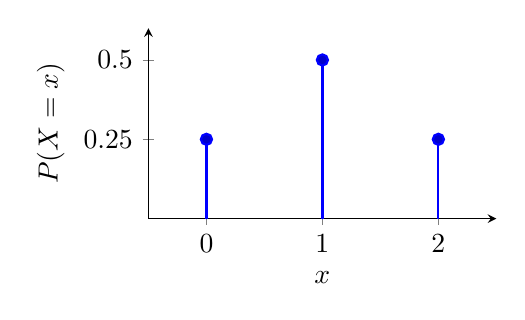
\begin{tikzpicture}
  \begin{axis}[
    ymin=0, ymax=0.6,
    xmin=-0.5, xmax=2.5,
    xtick={0,1,2},
    ytick={0.25,0.5},
    axis lines=left,
    width=6cm,
    height=4cm,
    xlabel={$x$},
    ylabel={$P(X = x)$},
    samples=3,
    domain=0:2,
    % enlargelimits=0.1,
    every axis plot/.append style={ultra thick}
  ]
  
  % Vertical lines
  \addplot+[ycomb, mark=*, blue, thick] coordinates {
    (0, 0.25)
    (1, 0.5)
    (2, 0.25)
  };

  \end{axis}
\end{tikzpicture}
\end{figure}


\end{frame}


%%%%%%%%%%%%%%%%%%%%%%%%%%%%%%%%%%%%%%%%%%%%%%%%%%%%%%%%%%%%%%%%%%%%%%%%%%%%%%%%
\begin{frame}{Continuous vs. Discrete random variable}

The examples on the previous slide are DISCRETE random variables (i.e. they take on a finite number of values)

\vspace{2ex}
Random variables can also be continuous. Examples:
\begin{itemize}
    \item Height of a random person selected in the population
    \item The time it takes you to commute to Hunter
    \item The temperature in Central Park at 10AM
\end{itemize}

\vspace{2ex}
These random variables take on an uncountably infinite number of values (even within a small interval)
\begin{itemize}
    \item Because each point in an interval is infinitely small, non-zero probabilities for continuous random variables are generally expressed as ranges
\begin{align*}
    \PP (45 \text{ minutes} < \text{My commute} \leq 60 \text{ minutes})
\end{align*}
\end{itemize}
Similar to how we used the \textbf{PMF} to describe probabilities for discrete random variables, we can describe probabilities for continuous random variables using the \textbf{probability density function} (\textbf{PDF}).

\end{frame}

%%%%%%%%%%%%%%%%%%%%%%%%%%%%%%%%%%%%%%%%%%%%%%%%%%%%%%%%%%%%%%%%%%%%%%%%%%%%%%%%
\begin{frame}{Probability Density Function}

Suppose $X$ follows a normal distribution with mean $\mu$ and standard deviation $\sigma$. The PDF for $X$, $f_X$, looks like:
\begin{figure}[width=0.25\textwidth]
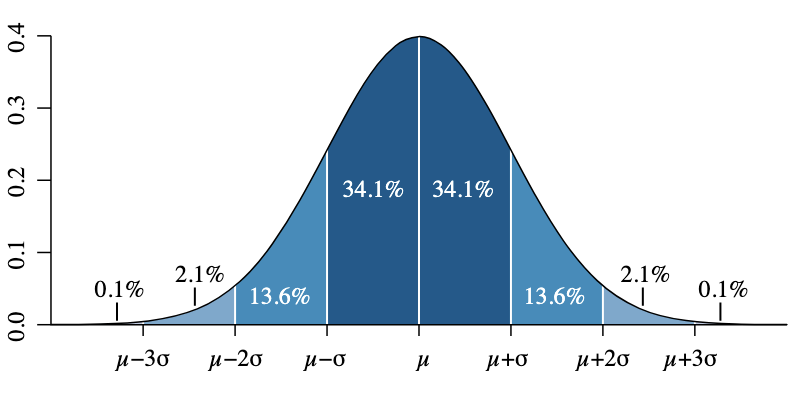
\includegraphics[scale=0.5]{img/normal_distribution.png}
\end{figure}
Then the probability that $X$ follows within one standard devation of the mean can be calculated by the area under the curve:
\begin{equation*}
    \PP (\mu - \sigma \leq X \leq \mu + \sigma) = 0.682
\end{equation*}


\end{frame}

%%%%%%%%%%%%%%%%%%%%%%%%%%%%%%%%%%%%%%%%%%%%%%%%%%%%%%%%%%%%%%%%%%%%%%%%%%%%%%%%
\begin{frame}{Continuous PDF}

In general, for some continuous random variable $X$ with density $f_X$, the probability is given by the area under the curve:
\begin{equation*}
    \PP (a \leq x \leq b) = \int_a^b f_X(x) dx
\end{equation*}

We won't make you do calculus in this class!  We'll focus on discrete random variables, but be aware that the infrastructure exists to deal with continuous random variables.

\end{frame}

%%%%%%%%%%%%%%%%%%%%%%%%%%%%%%%%%%%%%%%%%%%%%%%%%%%%%%%%%%%%%%%%%%%%%%%%%%%%%%%%
\begin{frame}{Cumulative distribution function (CDF)}

A cumulative distribution function is simply the probability that a random variable $X$ is less than or equal to some value:
\begin{equation*}
    F_X (x) = \PP (X \leq x)
\end{equation*}

\end{frame}


%%%%%%%%%%%%%%%%%%%%%%%%%%%%%%%%%%%%%%%%%%%%%%%%%%%%%%%%%%%%%%%%%%%%%%%%%%%%%%%%
\begin{frame}{Discrete CDF example}



\begin{figure}
\centering
\begin{subfigure}{0.4\textwidth}
\caption{Probability Mass Function}
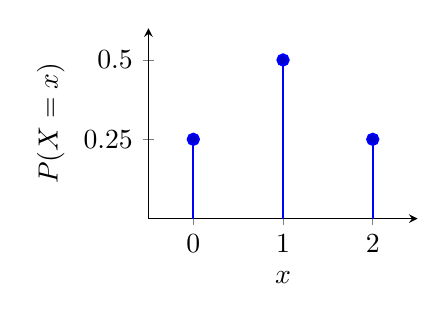
\begin{tikzpicture}
  \begin{axis}[
    ymin=0, ymax=0.6,
    xmin=-0.5, xmax=2.5,
    xtick={0,1,2},
    ytick={0.25,0.5},
    axis lines=left,
    width=5cm,
    height=4cm,
    xlabel={$x$},
    ylabel={$P(X = x)$},
    samples=3,
    domain=0:2,
    % enlargelimits=0.1,
    every axis plot/.append style={ultra thick}
  ]
  
  % Vertical lines
  \addplot+[ycomb, mark=*, blue, thick] coordinates {
    (0, 0.25)
    (1, 0.5)
    (2, 0.25)
  };

  \end{axis}
\end{tikzpicture}
\end{subfigure}

\hspace{3ex}

\begin{subfigure}{0.4\textwidth}
\caption{Cumulative Distribution Function}
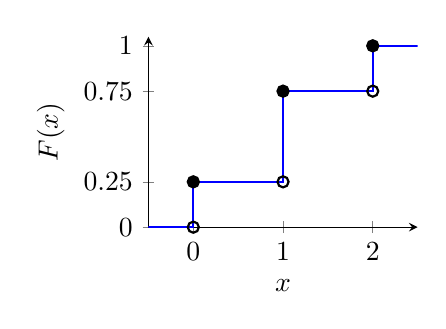
\begin{tikzpicture}
  \begin{axis}[
    axis x line=bottom,
    axis y line=left,
    xmin=-0.5, xmax=2.5,
    ymin=0, ymax=1.05,
    xtick={0,1,2},
    ytick={0,0.25,0.75,1},
    width=5cm,
    height=4cm,
    xlabel={$x$},
    ylabel={$F(x)$},
  ]
    % Step plot of CDF
    \addplot+[const plot, no marks, thick] coordinates {
      (-0.5, 0)
      (0, 0.25)
      (1, 0.75)
      (2, 1)
      (2.5, 1)
    };
    % Closed dots at jumps
    \addplot[only marks, mark=*, thick] coordinates {
      (0, 0.25)
      (1, 0.75)
      (2, 1)
    };
    % Open dots at left-hand limits (just before each jump)
    \addplot[only marks, mark=o, thick] coordinates {
      (0, 0)
      (1, 0.25)
      (2, 0.75)
    };
  \end{axis}
\end{tikzpicture}
\end{subfigure}
\end{figure}

\end{frame}

%%%%%%%%%%%%%%%%%%%%%%%%%%%%%%%%%%%%%%%%%%%%%%%%%%%%%%%%%%%%%%%%%%%%%%%%%%%%%%%%
\begin{frame}{Continuous CDF}

\begin{figure}
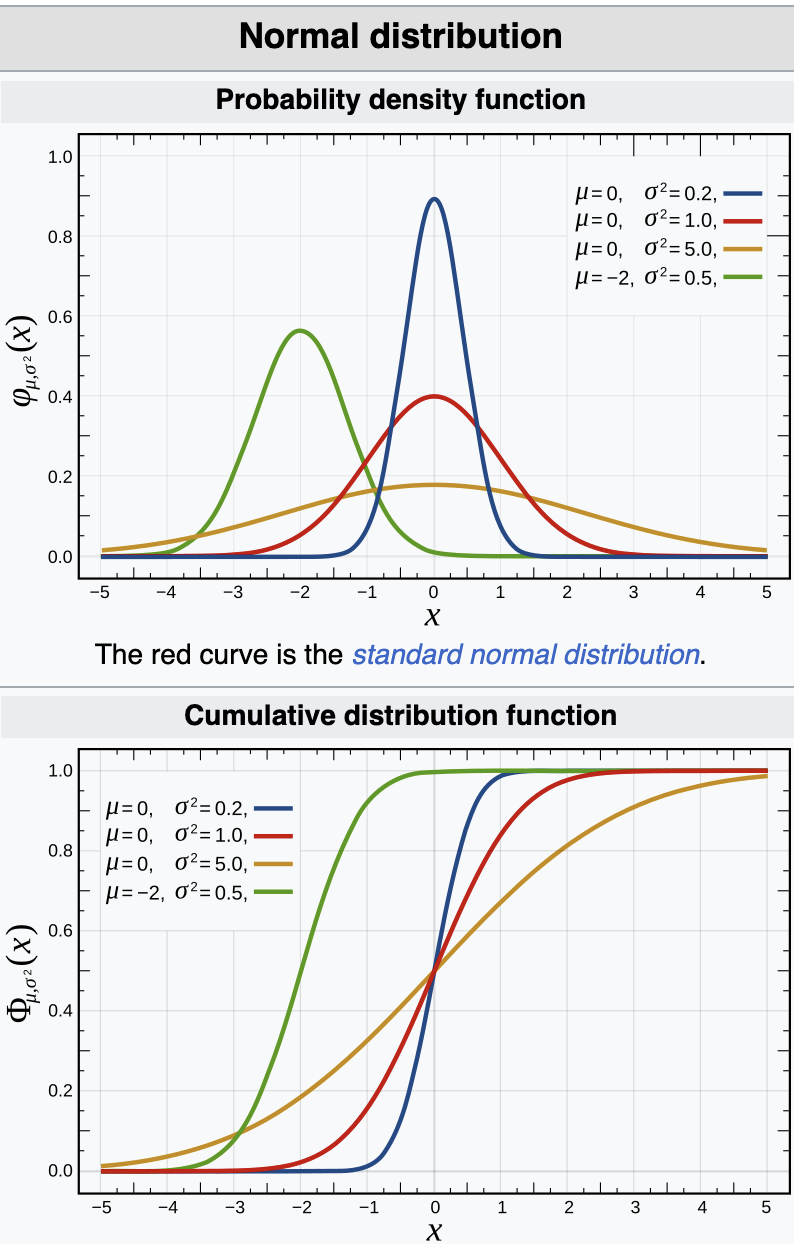
\includegraphics[scale=0.35]{img/normal_cdf.png}
\end{figure}

\end{frame}